% !TEX program = pdflatex
\documentclass[aspectratio=169,10pt]{beamer}

% ── Theme & colours ───────────────────────────────────────────
\usetheme[progressbar=frametitle,block=fill]{metropolis}
\definecolor{brandcolor}{HTML}{2C3E50}
\definecolor{accentcolor}{HTML}{800020}
\definecolor{lightcolor}{HTML}{F8F9F9}
\definecolor{darkgray}{HTML}{2C3E50}
\definecolor{lightgray}{HTML}{F2F3F4}
\definecolor{gray}{HTML}{7F8C8D}
\definecolor{successgreen}{HTML}{27AE60}
\definecolor{warnred}{HTML}{E74C3C}

\setbeamercolor{normal text}{fg=darkgray,bg=white}
\setbeamercolor{alerted text}{fg=warnred}
\setbeamercolor{example text}{fg=successgreen}
\setbeamercolor{progress bar}{fg=accentcolor,bg=lightgray}
\setbeamercolor{title separator}{fg=accentcolor,bg=lightgray}
\setbeamercolor{progress bar in section page}{fg=accentcolor}
\setbeamercolor{frametitle}{bg=brandcolor,fg=white}
\setbeamercolor{title}{fg=brandcolor}
\setbeamercolor{block title}{bg=brandcolor,fg=white}
\setbeamercolor{block body}{bg=lightcolor,fg=darkgray}
\setbeamercolor{block title alerted}{bg=warnred,fg=white}
\setbeamercolor{block body alerted}{bg=warnred!10,fg=darkgray}
\setbeamercolor{block title example}{bg=successgreen,fg=white}
\setbeamercolor{block body example}{bg=successgreen!10,fg=darkgray}

% ── Fonts ─────────────────────────────────────────────────────
\usepackage[T1]{fontenc}
\usepackage{lmodern}
\usepackage{microtype}

% ── Packages ──────────────────────────────────────────────────
\usepackage{booktabs}
\usepackage{array}
\usepackage{tabularx}
\usepackage{colortbl}
\usepackage{graphicx}
\graphicspath{{../../notebooks/plots/}}
\usepackage{amsmath}
\usepackage{multicol}

% ── Remove navigation symbols ─────────────────────────────────
\setbeamertemplate{navigation symbols}{}

% ── Footline ──────────────────────────────────────────────────
% Metropolis handles slide numbers automatically.

% ── Table row colours ─────────────────────────────────────────
\rowcolors{2}{white}{lightcolor}

% ── Custom commands ───────────────────────────────────────────
\newcommand{\metricbox}[3]{%
  \fcolorbox{accentcolor}{lightcolor}{%
    \parbox[c][1.6cm][c]{2.6cm}{\centering
      {\small\color{gray}#1}\\[3pt]
      {\Large\bfseries\color{brandcolor}#2}\\[2pt]
      {\tiny\color{gray}#3}%
    }%
  }%
}

% ═══════════════════════════════════════════════════════════════
\title{\textbf{Predicting Customer Order Value}\\[6pt]
       \large for an E-Commerce Platform}
\subtitle{Business Analytics --- Project Presentation}
\author{
  \textbf{Group 13}\\[4pt]
  \small Nguyen Huy Hoang 20251325M\\
  \small Nguyen Luong Quynh Trang 20252761M\\
  \small Tran Tien Dung 20252574M\\
  \small Tran Manh Tien 20252762M\\
  \small Bui Duc Phan Hoang 20252004M
}
\institute{Brazilian E-Commerce Public Dataset (Olist)}
\date{\today}

\begin{document}

% ── Title slide ───────────────────────────────────────────────
\begin{frame}
  \titlepage
\end{frame}

% ── Agenda ────────────────────────────────────────────────────
\begin{frame}{Agenda}
  \tableofcontents
\end{frame}

% ═══════════════════════════════════════════════════════════════
\section{Problem Statement}

\begin{frame}{Business Problem}
  \begin{columns}[T]
    \column{0.55\textwidth}
    \textbf{The challenge:} E-commerce platforms rely on
    \emph{population-level averages} for operational decisions, obscuring
    substantial variation between individual orders.

    \vspace{8pt}
    \textbf{Operational decisions affected:}
    \begin{itemize}
      \item Shipping tier selection
      \item Upsell recommendation timing
      \item Fraud review prioritisation
      \item Promotional targeting
    \end{itemize}

    \column{0.42\textwidth}
    \begin{block}{Objective}
      Replace population-level averages with
      \textbf{individual-level predictions} of order value.
    \end{block}
    \vspace{4pt}
    \begin{alertblock}{Research Question}
      Given a customer's profile and session behaviour, what is the
      expected order value, and which factors drive it?
    \end{alertblock}
  \end{columns}
\end{frame}

\begin{frame}{Business Value}
  Accurate order value predictions enable three categories of action:

  \vspace{10pt}
  \begin{columns}[T]
    \column{0.31\textwidth}
    \centering
    \metricbox{Upsell}{Dynamic}{Calibrated to\\predicted value tier}
    \vspace{8pt}

    \column{0.31\textwidth}
    \centering
    \metricbox{Shipping}{Optimised}{Matched to\\order magnitude}
    \vspace{8pt}

    \column{0.31\textwidth}
    \centering
    \metricbox{Promotions}{Targeted}{Directed to highest\\incremental revenue}
  \end{columns}

  \vspace{12pt}
  \begin{exampleblock}{Projected Monthly Return}
    \textbf{R\$16{,}140/month} ($\sim$R\$193{,}680 annually) from dynamic
    upsell profit and insurance compliance savings, based on 10{,}000
    monthly orders at R\$138 AOV.
  \end{exampleblock}
\end{frame}

% ═══════════════════════════════════════════════════════════════
\section{Data Strategy}

\begin{frame}{Data Foundation: Olist Dataset}
  \begin{columns}[T]
    \column{0.5\textwidth}
    \textbf{Nine relational tables:}
    \begin{itemize}
      \item 99{,}441 orders
      \item 112{,}650 line items
      \item 32{,}951 products
      \item 3{,}095 sellers
      \item 1{,}000{,}163 geolocation records
    \end{itemize}

    \vspace{6pt}
    \textbf{Period:} September 2016 -- October 2018

    \column{0.47\textwidth}
    \begin{block}{Critical Gap}
      Olist captures \emph{what} was purchased but not \emph{how} the
      customer arrived at that purchase.

      \vspace{4pt}
      \small No session data, clickstream, demographics, or loyalty
      information.
    \end{block}
  \end{columns}
\end{frame}

\begin{frame}{Synthetic Behavioural Data}
  Three tables generated following an ERD-aligned schema:

  \vspace{6pt}
  \small
  \rowcolors{2}{white}{lightcolor}
  \begin{tabularx}{\textwidth}{l r X}
    \toprule
    \rowcolor{brandcolor}
    \textcolor{white}{\textbf{Table}} & \textcolor{white}{\textbf{Rows}} & \textcolor{white}{\textbf{Contents}} \\
    \midrule
    \texttt{customer\_profile} & 96{,}096 & Demographics, income, loyalty tier, device preference \\
    \texttt{sessions}          & 99{,}441 & Device, browser, OS, traffic source, session timing, coupons \\
    \texttt{session\_activity} & 763{,}850 & Clickstream: page views, searches, cart additions, checkout \\
    \bottomrule
  \end{tabularx}

  \vspace{10pt}
  \begin{alertblock}{Design Principle: Value-Conditioned Generation}
    Each synthetic feature is conditioned on the real order value via
    $v_s = z\text{-score}(\log(1+y))$, ensuring genuine predictive
    signal---not random noise.
  \end{alertblock}
\end{frame}

\begin{frame}{Value-Conditioned Correlation Design}
  \small
  \rowcolors{2}{white}{lightcolor}
  \begin{tabularx}{\textwidth}{l c X}
    \toprule
    \rowcolor{brandcolor}
    \textcolor{white}{\textbf{Feature}} & \textcolor{white}{\textbf{Target Effect}} & \textcolor{white}{\textbf{Rationale}} \\
    \midrule
    Monthly income      & $r \approx 0.51$     & Higher income $\rightarrow$ higher spending capacity \\
    Loyalty tier        & $2.5\times$ AOV spread & Loyal customers trust platform, spend more \\
    Traffic source      & Email +64\% vs Google  & Email = loyal repeat; Google = acquisition \\
    Device type         & Desktop +7\%           & Desktop = deliberate shopping, larger carts \\
    Session engagement  & $r \approx 0.2$        & More deliberation $\rightarrow$ higher-value orders \\
    \midrule
    \rowcolor{lightgray}
    Gender, education   & $r \approx 0$ (indep.) & No realistic causal link to individual order value \\
    \bottomrule
  \end{tabularx}

  \vspace{8pt}
  \textbf{Leakage prevention:} Residual noise ($\sigma = 0.5$--$0.7$) ensures
  no single synthetic feature exceeds $r = 0.5$; model $R^{2}$ from synthetic
  features alone $\approx 0.10$--$0.25$.
\end{frame}

% ═══════════════════════════════════════════════════════════════
\section{Exploratory Data Analysis}

\begin{frame}{Target Distribution}
  \begin{columns}[T]
    \column{0.55\textwidth}
    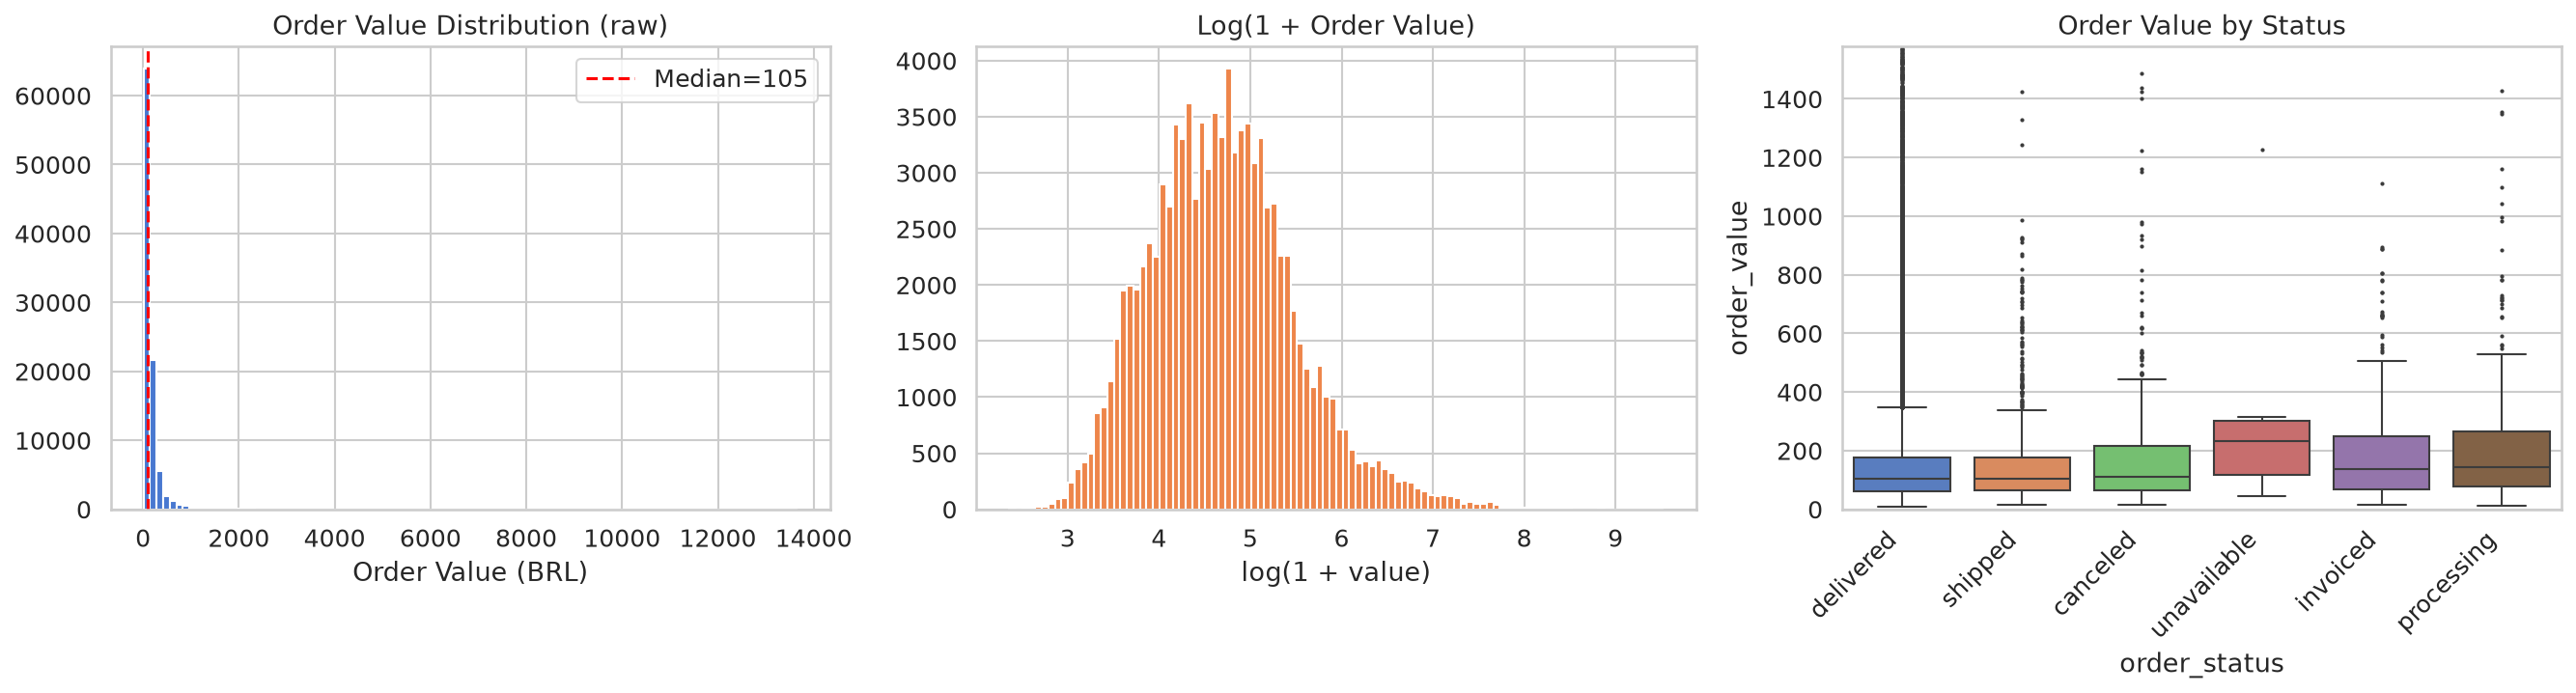
\includegraphics[width=\textwidth]{01_target_distribution.png}

    \column{0.42\textwidth}
    \textbf{Key statistics:}
    \begin{itemize}
      \item Median: R\$105
      \item Mean: R\$160
      \item Max: R\$13{,}664
      \item Skewness: 9.37
    \end{itemize}

    \vspace{8pt}
    \begin{block}{Transformation}
      $\log(1+y)$ reduces skewness to \textbf{0.17}, producing a
      near-normal distribution suitable for regression.
    \end{block}
  \end{columns}
\end{frame}

\begin{frame}{Value Drivers}
  \begin{columns}[T]
    \column{0.48\textwidth}
    \centering
    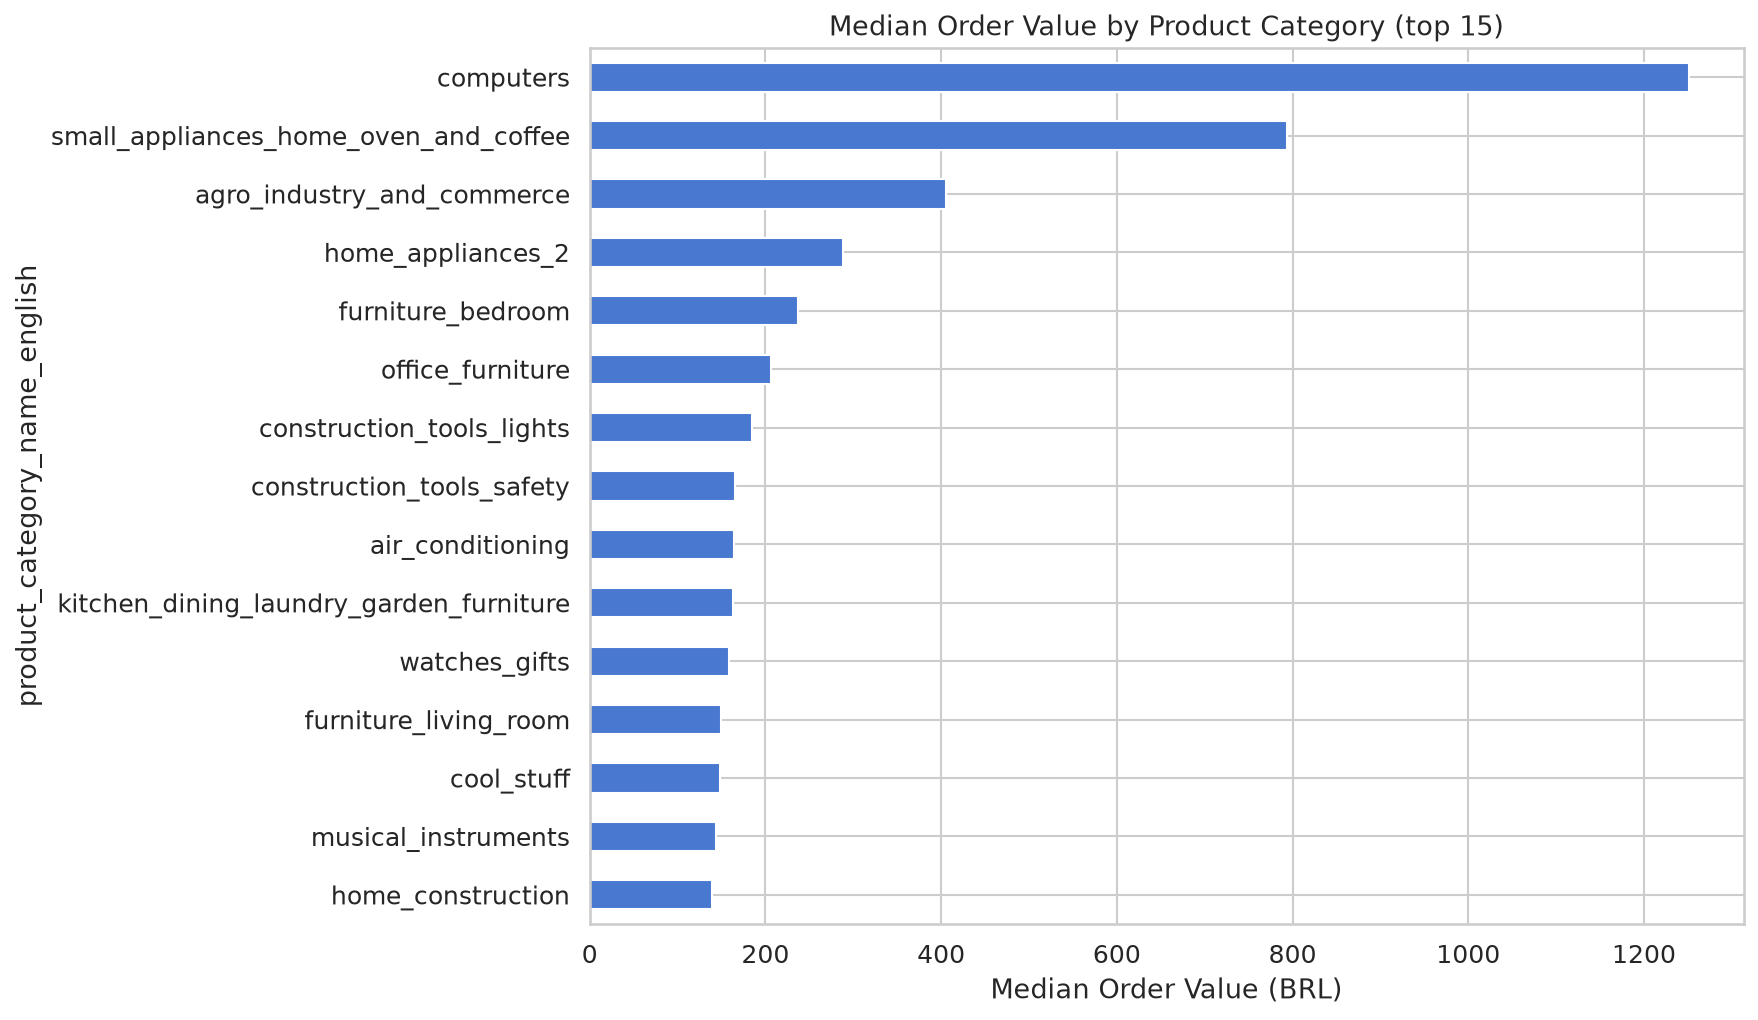
\includegraphics[width=0.95\textwidth]{02_value_by_category.png}\\[4pt]
    {\small\textbf{40-fold} variation across categories}

    \column{0.48\textwidth}
    \centering
    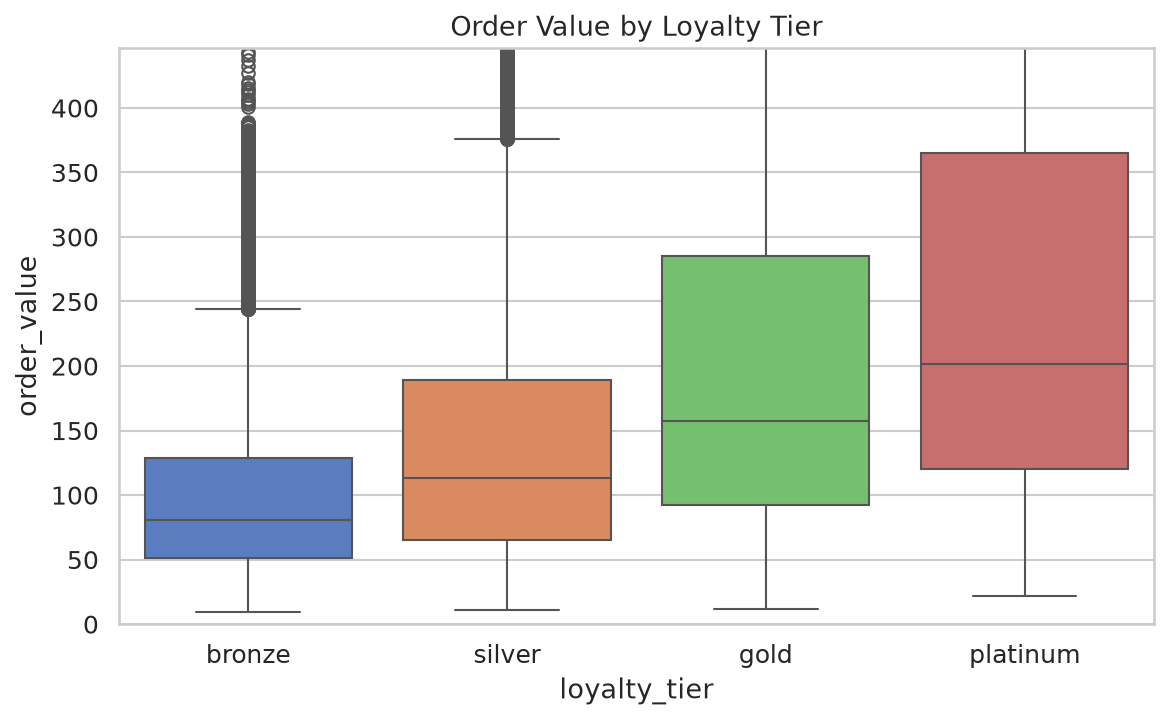
\includegraphics[width=0.85\textwidth]{05_value_by_loyalty.png}\\[4pt]
    {\small\textbf{2.5$\times$} spread: bronze $\rightarrow$ platinum}
  \end{columns}
\end{frame}

\begin{frame}{Session Behavior \& Multicollinearity}
  \begin{columns}[T]
    \column{0.48\textwidth}
    \centering
    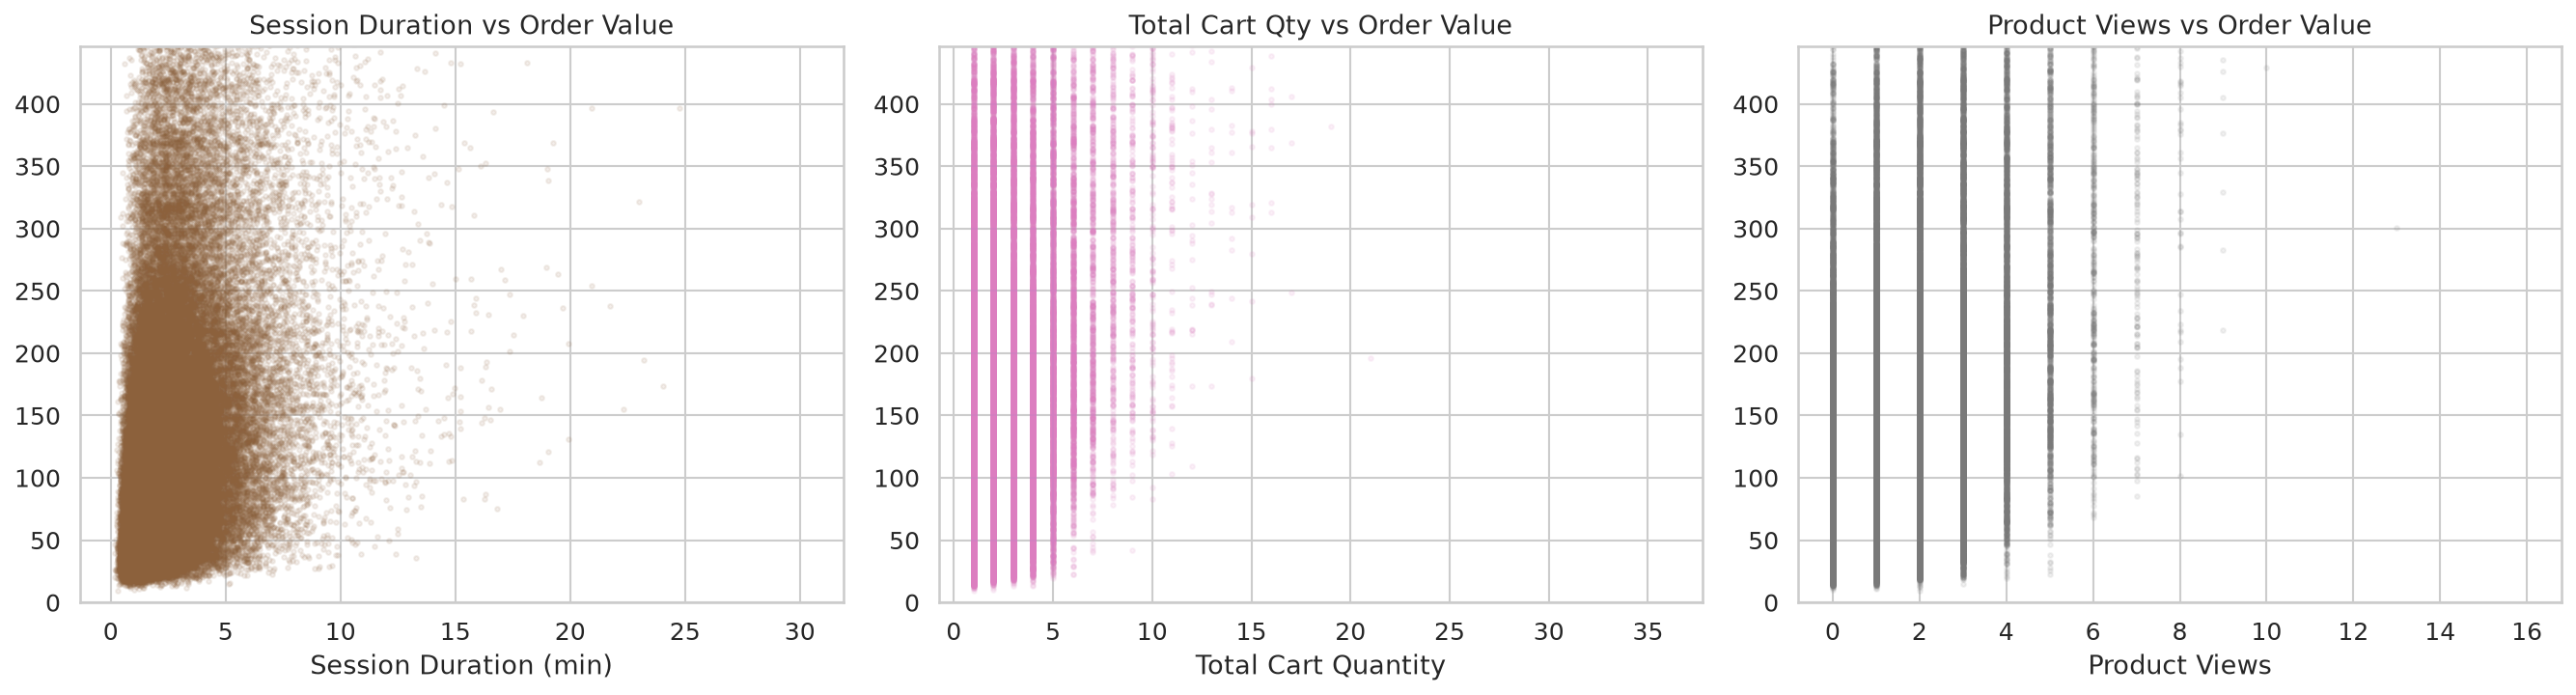
\includegraphics[width=1.0\textwidth]{08_session_behavior_vs_value.png}\\[4pt]
    {\small\textbf{Session Behavior:} Duration and cart additions scale with higher-value baskets.}

    \column{0.48\textwidth}
    \centering
    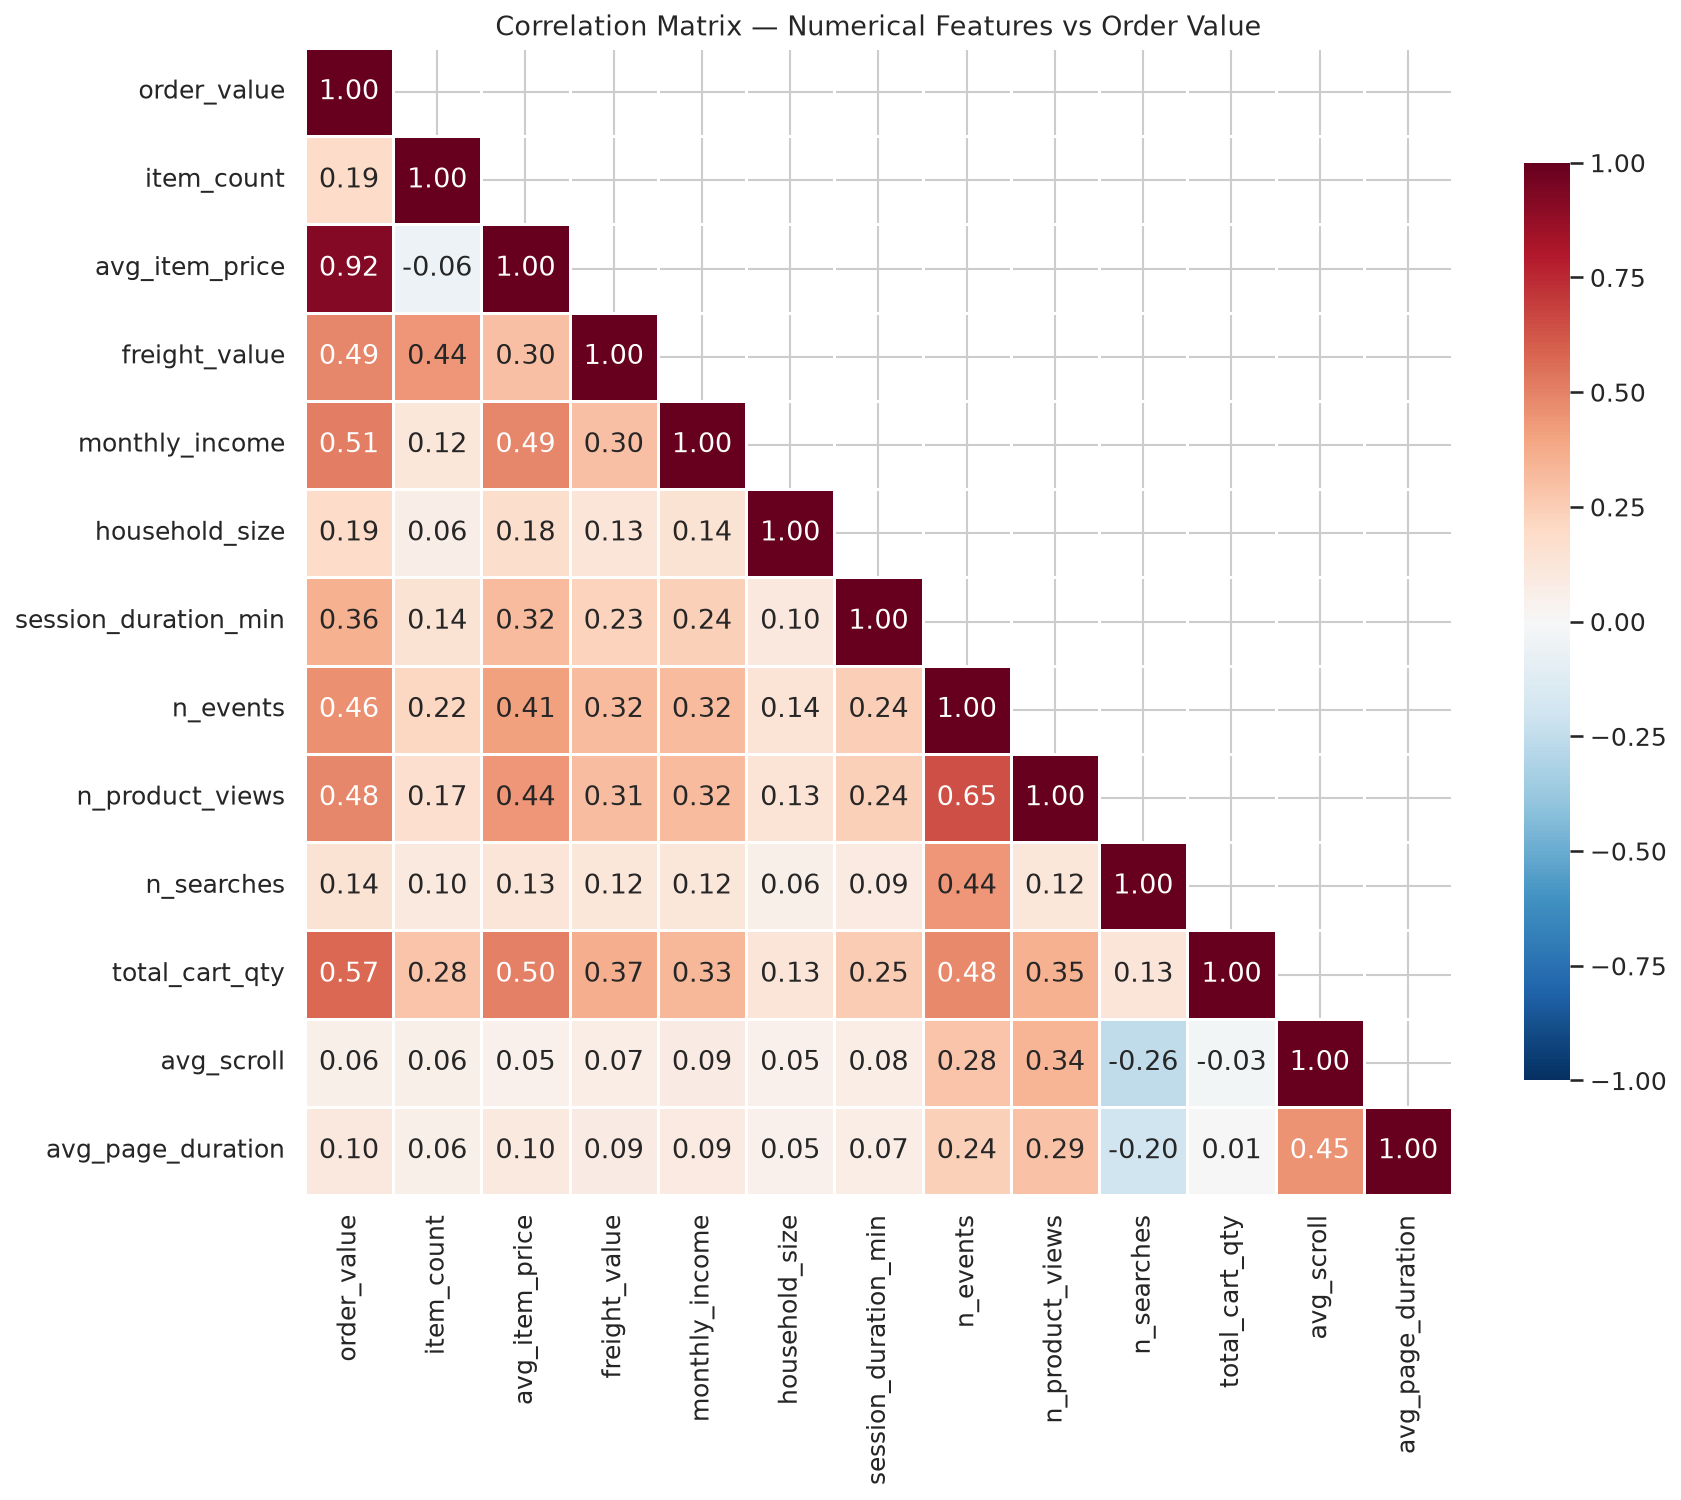
\includegraphics[width=1.0\textwidth]{09_correlation_heatmap.png}\\[4pt]
    {\small\textbf{Correlation:} No independent features exceed $|r|=0.7$, mitigating multicollinearity.}
  \end{columns}
\end{frame}

% ═══════════════════════════════════════════════════════════════
\section{Feature Engineering}

\begin{frame}{From 73 Columns to 182 Features}
  \small
  \rowcolors{2}{white}{lightcolor}
  \begin{tabularx}{\textwidth}{l r X}
    \toprule
    \rowcolor{brandcolor}
    \textcolor{white}{\textbf{Group}} & \textcolor{white}{\textbf{Count}} & \textcolor{white}{\textbf{Examples}} \\
    \midrule
    One-hot categoricals    & 131 & Device, browser, OS, traffic, loyalty, category, seller state \\
    Scaled numericals       &  47 & Income, session duration, geolocation, haversine distance, RFM \\
    Target-encoded          &   3 & IP region, campaign name, seller state (smoothed) \\
    Derived interactions    &  16 & Income$\times$loyalty, cart conversion, engagement rate \\
    Boolean flags           &   3 & Logged-in, marketing opt-in, coupon applied \\
    \midrule
    \rowcolor{accentcolor!15}
    \textbf{Total}          & \textbf{182} & VIF analysis removed 3 collinear features \\
    \bottomrule
  \end{tabularx}

  \vspace{8pt}
  \textbf{Cleaning decisions:}
  \begin{itemize}
    \item 1{,}856 cancelled/unavailable orders removed
    \item 71 Portuguese category names translated
    \item Geolocation, seller reputation, regional price indices integrated
    \item \textbf{No winsorization}---full value range preserved; outlier
          robustness via $L_{1}$ loss
  \end{itemize}
\end{frame}

% ═══════════════════════════════════════════════════════════════
\section{Modelling}

\begin{frame}{Model Comparison}
  \textbf{Split:} Time-based at 2018-04-01 (65{,}124 train / 32{,}460 test)

  \vspace{8pt}
  \small
  \rowcolors{2}{white}{lightcolor}
  \begin{tabular}{l ccccc}
    \toprule
    \rowcolor{brandcolor}
    \textcolor{white}{\textbf{Model}} & \textcolor{white}{$\boldsymbol{R^{2}}$}
      & \textcolor{white}{\textbf{MAE}} & \textcolor{white}{\textbf{WAPE}}
      & \textcolor{white}{\textbf{MedAPE}} & \textcolor{white}{\textbf{MAPE}} \\
    \midrule
    Linear Regression & 0.74 & R\$318 & 193\% & 27\% & 34\% \\
    Ridge             & 0.74 & R\$318 & 193\% & 27\% & 34\% \\
    Lasso             & 0.64 & R\$141 &  86\% & 32\% & 42\% \\
    Random Forest     & 0.79 &  R\$49 &  30\% & 22\% & 30\% \\
    \rowcolor{accentcolor!20}
    \textbf{XGBoost ($L_1$)} & \textbf{0.80} & \textbf{R\$48} & \textbf{29\%} & \textbf{21\%} & \textbf{28\%} \\
    LightGBM (MAE)    & 0.80 &  R\$48 &  29\% & 22\% & 29\% \\
    \bottomrule
  \end{tabular}

  \vspace{8pt}
  \begin{itemize}
    \item $L_{2}$-based models: extreme MAE due to outlier sensitivity
    \item Tree-based + $L_{1}$: MAE $<$ R\$50
    \item \textbf{XGBoost selected:} best MedAPE (21\%)
  \end{itemize}
\end{frame}

\begin{frame}{Feature Importance: Validation of Synthetic Data}
  \begin{columns}[T]
    \column{0.52\textwidth}
    \small
    \rowcolors{2}{white}{lightcolor}
    \begin{tabular}{c l c}
      \toprule
      \rowcolor{brandcolor}
      \textcolor{white}{\#} & \textcolor{white}{\textbf{Feature}} & \textcolor{white}{\textbf{Imp.}} \\
      \midrule
      1 & income $\times$ loyalty & 14.0\% \\
      2 & session event count     &  8.8\% \\
      3 & cart additions          &  8.8\% \\
      4 & product views           &  5.2\% \\
      5 & total cart quantity     &  5.1\% \\
      6 & payment installments    &  3.5\% \\
      7 & category: telephony     &  2.7\% \\
      8 & log income              &  2.6\% \\
      9 & category: electronics   &  2.4\% \\
      10 & loyalty: bronze        &  2.3\% \\
      \bottomrule
    \end{tabular}

    \column{0.45\textwidth}
    \begin{alertblock}{Key Finding}
      \textbf{13 of 20} top features are synthetic behavioural features.

      \vspace{4pt}
      The value-conditioned generation produces data the model finds
      \emph{genuinely predictive}.
    \end{alertblock}

    \vspace{6pt}
    \begin{block}{Discriminative Power}
      Bronze mobile, 1 item: \textbf{R\$83}\\
      Platinum desktop, 5 items: \textbf{R\$520}\\[4pt]
      \centering $6.3\times$ spread
    \end{block}
  \end{columns}
\end{frame}

\begin{frame}{Feature Importance (Top 20)}
  \centering
  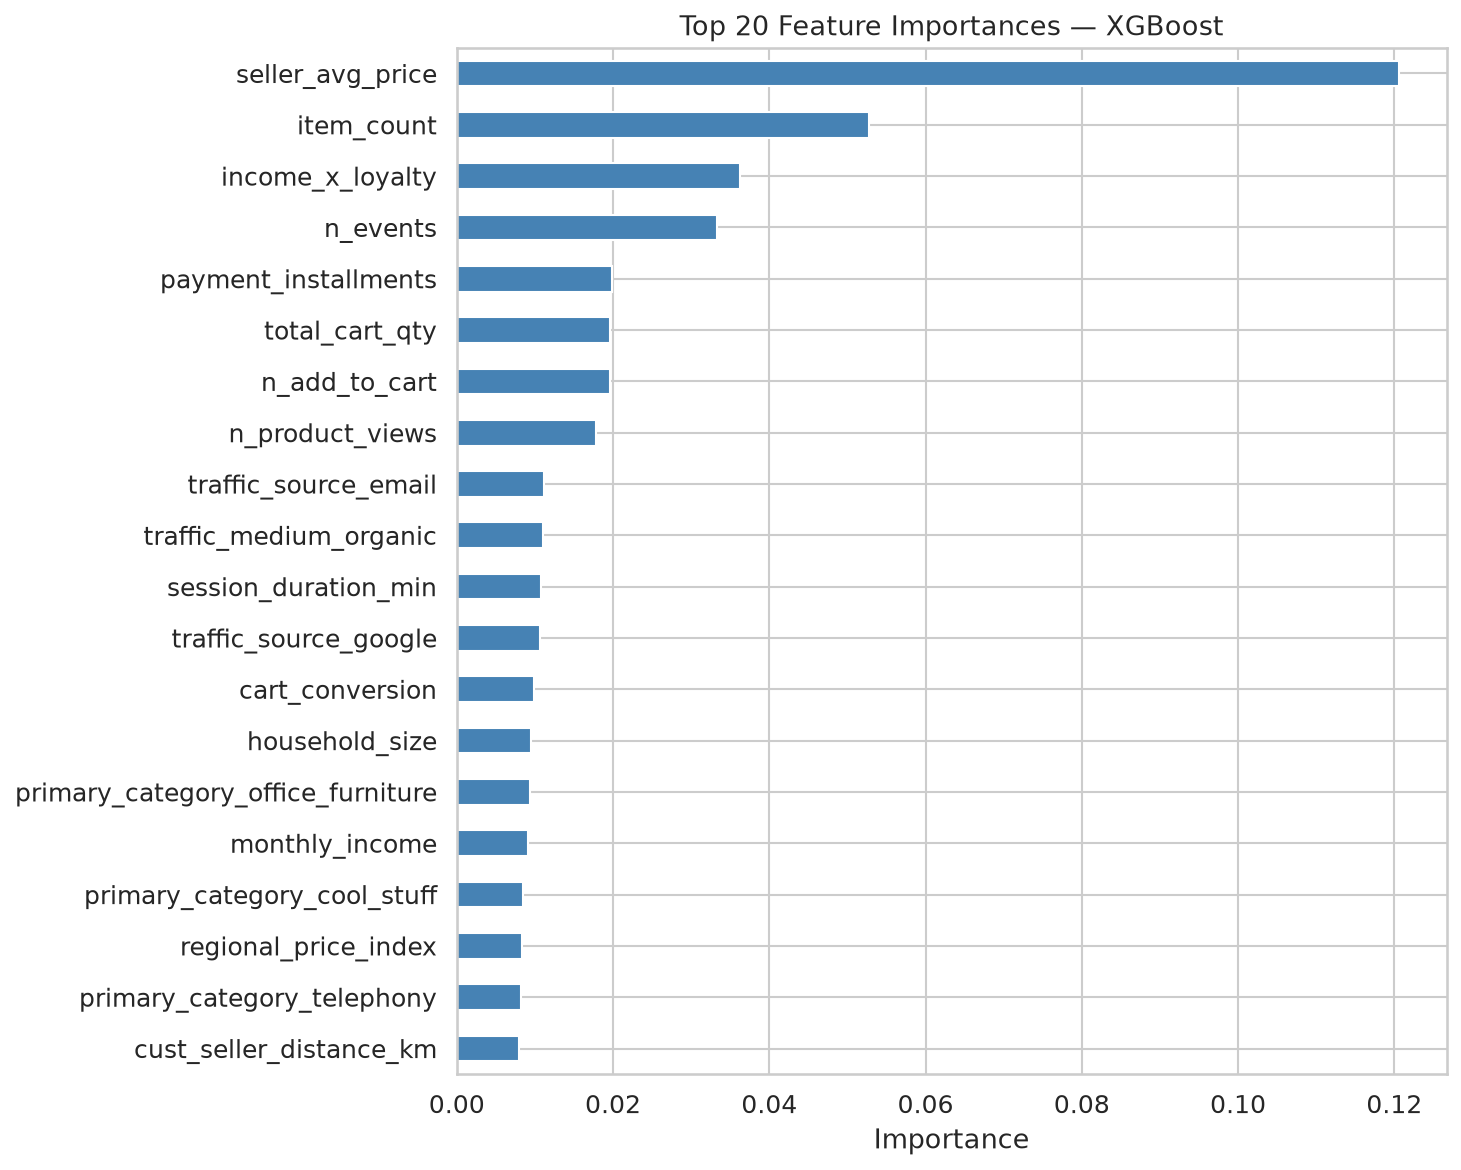
\includegraphics[width=0.85\textwidth]{feature_importance.png}
\end{frame}

\begin{frame}{Residual Analysis}
  \begin{columns}[T]
    \column{0.45\textwidth}
    \textbf{Log-Space Diagnosis}
    \begin{itemize}
      \item Normal distribution of residuals
      \item Homoscedasticity generally maintained
    \end{itemize}
    \textbf{Original Scale (BRL)}
    \begin{itemize}
      \item Errors naturally expand for extreme high-value orders
      \item Validates the choice of proportional KPI (WAPE, MAPE)
    \end{itemize}
    
    \column{0.5\textwidth}
    \centering
    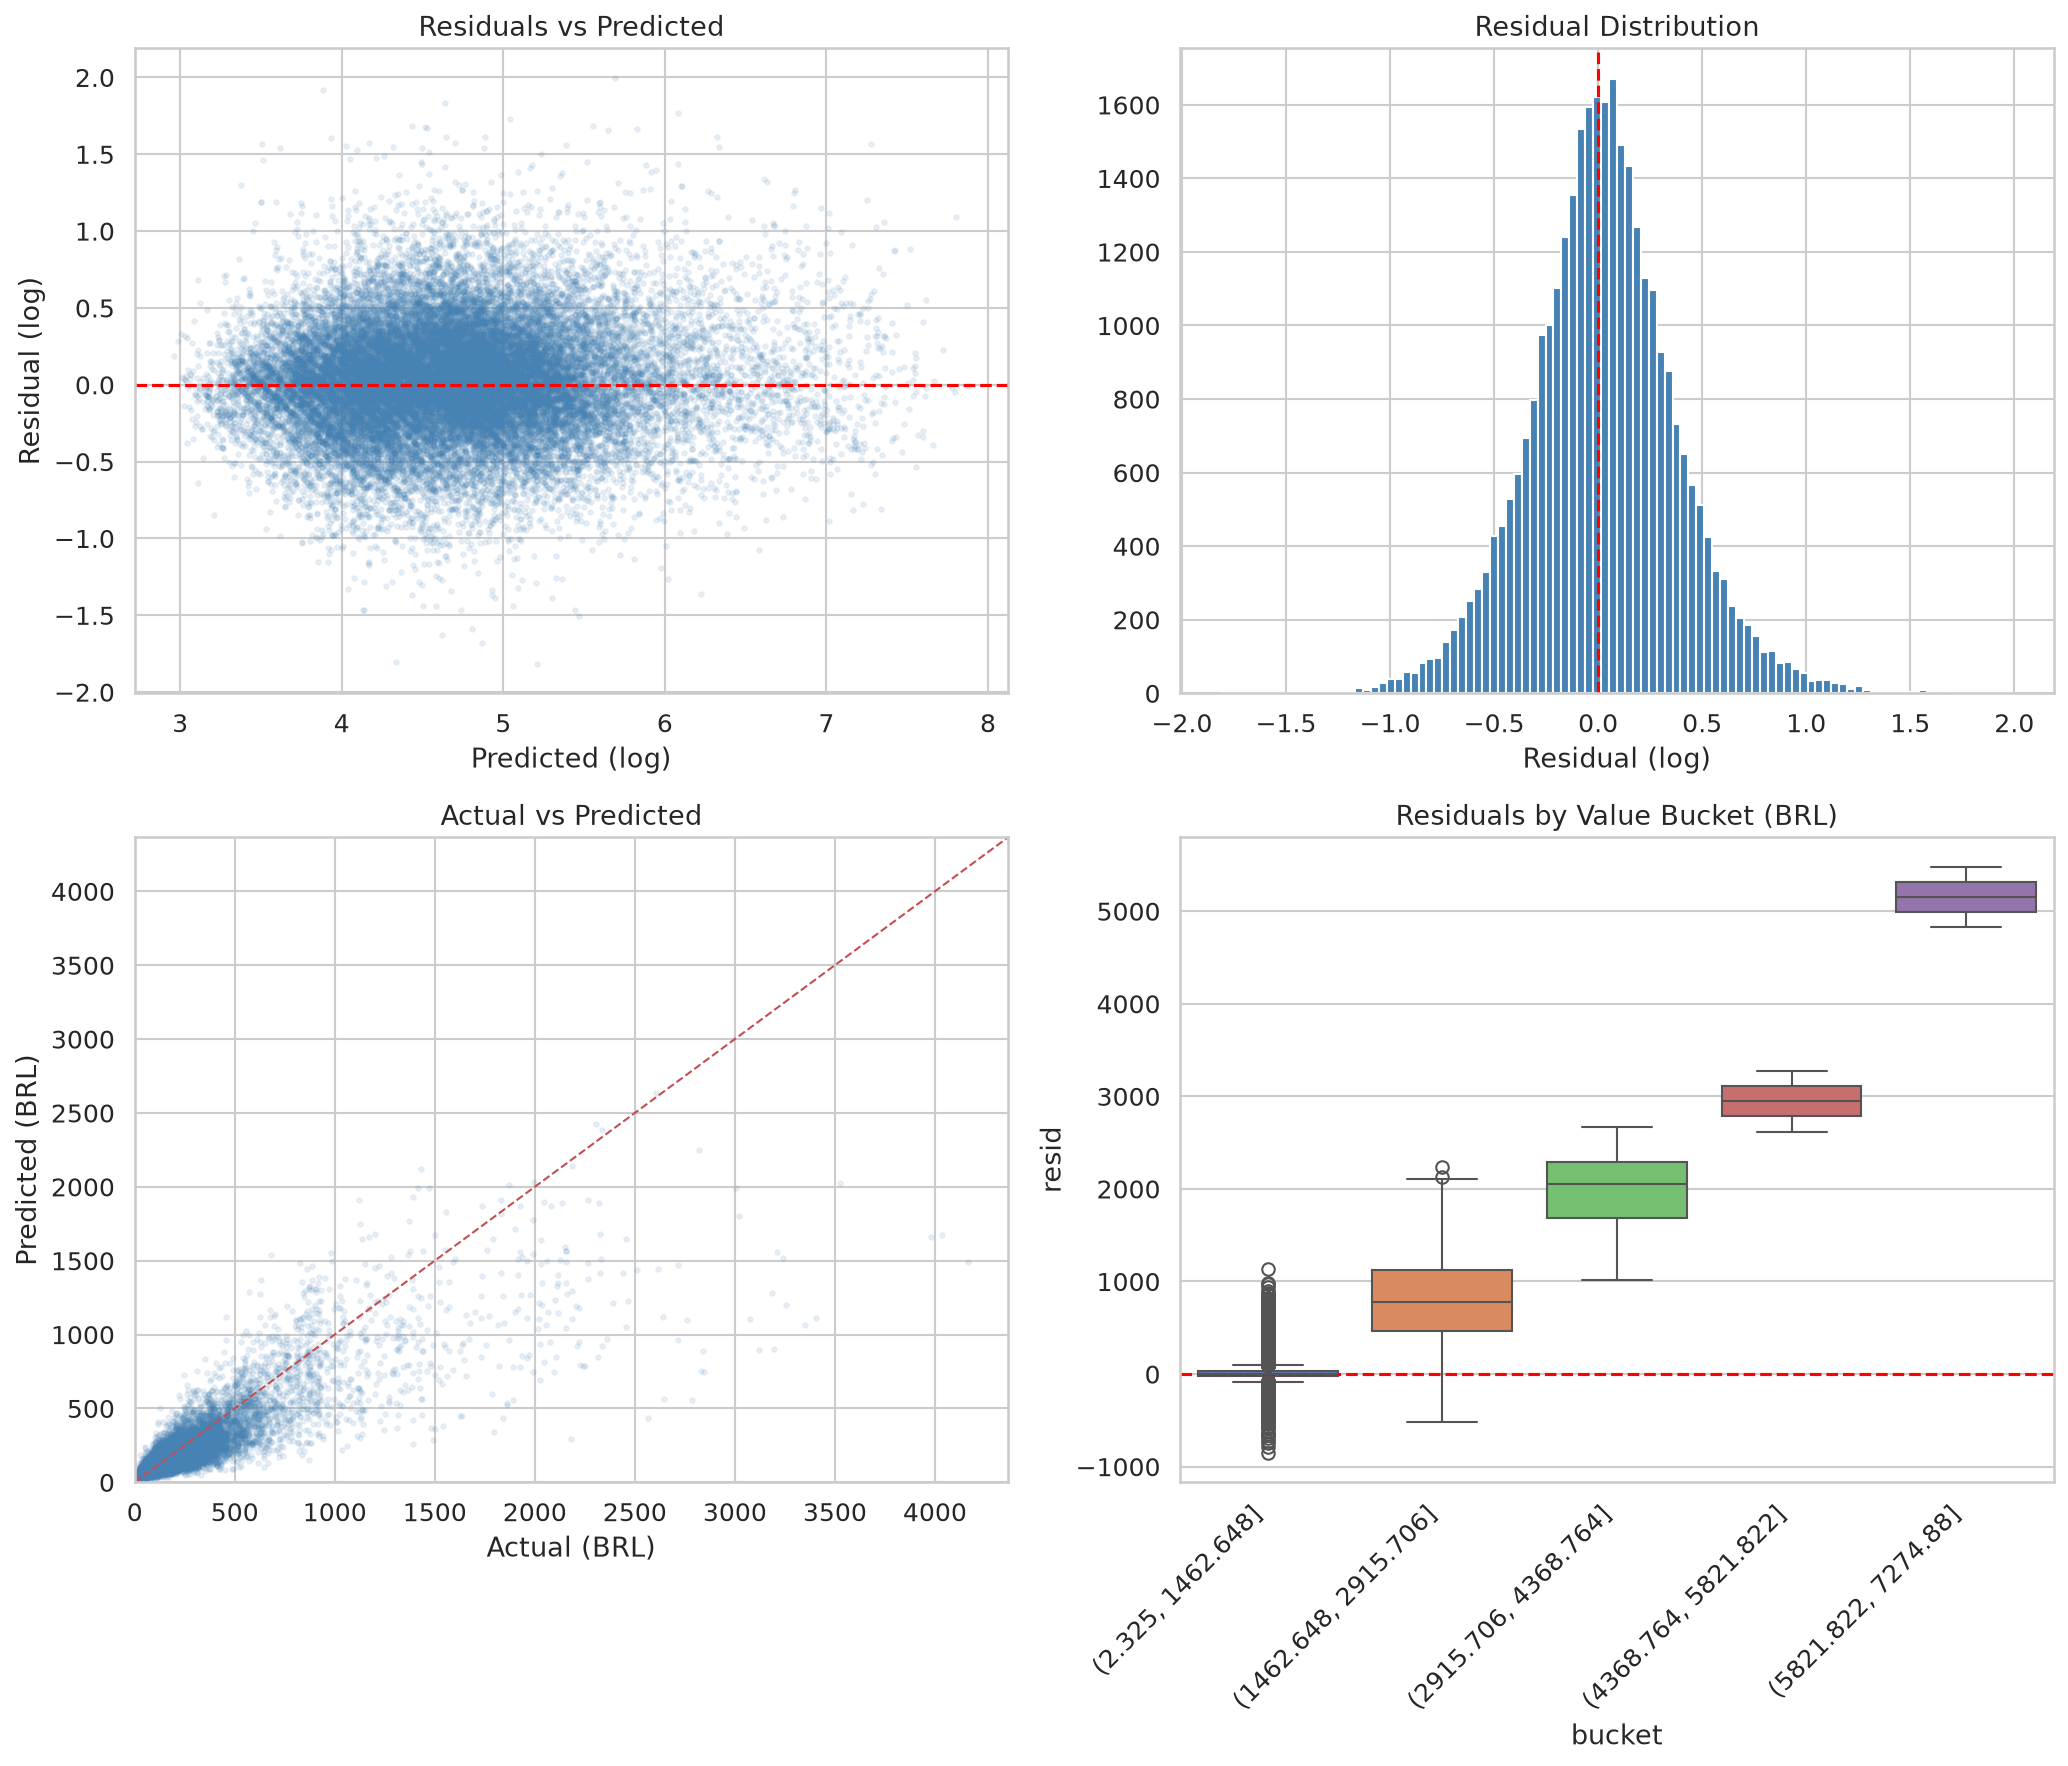
\includegraphics[width=1.0\textwidth]{residual_analysis.png}
  \end{columns}
\end{frame}


% ═══════════════════════════════════════════════════════════════
\section{Deployment \& Monitoring}

\begin{frame}{System Architecture}
  \begin{columns}[T]
    \column{0.48\textwidth}
    \textbf{Prediction API (FastAPI)}
    \begin{itemize}
      \item \texttt{POST /predict}: 30+ features $\rightarrow$ value + 80\% CI
      \item \texttt{GET /health}: liveness check
      \item Model + preprocessor serialised as single artifact
    \end{itemize}

    \vspace{8pt}
    \textbf{Interactive Demo (Streamlit)}
    \begin{itemize}
      \item Sidebar controls for all inputs
      \item Real-time business insights
      \item Standalone version for HF Spaces
    \end{itemize}

    \column{0.48\textwidth}
    \textbf{Monitoring}
    \begin{itemize}
      \item PSI drift detection per feature
      \item Evidently AI dashboards (3 reports)
      \item Retraining triggers:
        \begin{itemize}
          \item Feature PSI $> 0.25$
          \item Rolling 7-day WAPE $> 35\%$
        \end{itemize}
    \end{itemize}

    \vspace{8pt}
    \textbf{Deployment}
    \begin{itemize}
      \item Dockerfile for containerisation
      \item HuggingFace Spaces (Streamlit)
      \item \texttt{run\_pipeline.sh}: single-command E2E
    \end{itemize}
  \end{columns}
\end{frame}

% ═══════════════════════════════════════════════════════════════
\section{Business Recommendations}

\begin{frame}{Actionable Recommendations}
  \small
  \begin{enumerate}
    \item \textbf{Loyalty tier upgrade programmes}\\
          {\color{gray}$2.5\times$ AOV spread (bronze R\$82 $\rightarrow$
          platinum R\$202) --- largest single lever}

    \vspace{4pt}
    \item \textbf{Email channel investment}\\
          {\color{gray}64\% higher median AOV vs.\ Google organic; lower
          acquisition cost}

    \vspace{4pt}
    \item \textbf{Desktop experience optimisation}\\
          {\color{gray}7\% higher median AOV; critical for high-value
          categories}

    \vspace{4pt}
    \item \textbf{Real-time cart upsell triggers}\\
          {\color{gray}Cart additions rank \#3 in importance; target
          low-engagement sessions}

    \vspace{4pt}
    \item \textbf{Income-tier personalisation}\\
          {\color{gray}Income $\times$ loyalty = \#1 feature (14\%); use
          predicted tier for real-time segmentation}
  \end{enumerate}
\end{frame}

% ═══════════════════════════════════════════════════════════════
\section{Limitations \& Future Work}

\begin{frame}{Limitations and Future Directions}
  \begin{columns}[T]
    \column{0.48\textwidth}
    \textbf{Current Limitations}
    \begin{itemize}
      \item Synthetic correlations are \emph{designed}, not observed
      \item No product-level pricing features
      \item 97\% single-order customers (limited longitudinal data)
      \item KPI targets not fully met
    \end{itemize}

    \vspace{8pt}
    \small
    \rowcolors{2}{white}{lightcolor}
    \begin{tabular}{lcc}
      \toprule
      \rowcolor{brandcolor}
      \textcolor{white}{\textbf{KPI}} & \textcolor{white}{\textbf{Target}} & \textcolor{white}{\textbf{Actual}} \\
      \midrule
      MAE    & $<$R\$25 & R\$48 \\
      WAPE   & $<$16\%  & 29\% \\
      MedAPE & $<$12\%  & 22\% \\
      MAPE   & $<$15\%  & 29\% \\
      \bottomrule
    \end{tabular}

    \column{0.48\textwidth}
    \textbf{Future Directions}
    \begin{itemize}
      \item Integrate real clickstream data
      \item Add product-level pricing features
      \item Sequence models (LSTM / Transformers) for clickstream
      \item External data: competitor pricing, macroeconomic indicators
    \end{itemize}

    \vspace{8pt}
    \begin{block}{Path to KPI Targets}
      Product-level pricing + sequence architectures are expected to
      close the majority of the remaining gap.
      
    \end{block}
  \end{columns}
\end{frame}


% ═══════════════════════════════════════════════════════════════
\section{Summary}

\begin{frame}{Summary}
  \begin{columns}[T]
    \column{0.48\textwidth}
    \textbf{Results}
    \vspace{6pt}

    \metricbox{$R^{2}$}{0.79}{Variance explained}
    \hspace{4pt}
    \metricbox{MAE}{R\$48}{Mean absolute error}

    \vspace{8pt}

    \metricbox{WAPE}{29\%}{Weighted abs.\ pct.\ error}
    \hspace{4pt}
    \metricbox{MedAPE}{22\%}{Median abs.\ pct.\ error}

    \column{0.48\textwidth}
    \textbf{Key Contributions}
    \begin{itemize}
      \item Value-conditioned synthetic data with validated predictive power
      \item 182-feature engineering pipeline
      \item End-to-end reproducible system
      \item FastAPI + Streamlit + Docker deployment
      \item PSI + Evidently monitoring
      \item 43 tests, single-command pipeline
    \end{itemize}

    \vspace{6pt}
    \begin{exampleblock}{Bottom Line}
      Synthetic behavioural features drive 13/20 top predictions---validating
      the data generation design.
    \end{exampleblock}
  \end{columns}
\end{frame}

% ── Closing slide ─────────────────────────────────────────────
\begin{frame}{}
  \vfill
  \centering
  {\LARGE\bfseries\color{brandcolor} Thank You}\\[12pt]
  {\large\color{accentcolor} Questions \& Discussion}\\[20pt]
  {\small\color{gray}
    \textbf{Repository:} \texttt{github.com/alitonia/customer\_value\_prediction}\\[4pt]
    \textbf{Live Demo:} \texttt{huggingface.co/spaces/alitonia/customer\_value\_prediction}\\[4pt]
    Brazilian E-Commerce Public Dataset (Olist) --- 99{,}441 orders
  }
  \vfill
\end{frame}

\end{document}
